\documentclass[a4paper]{article}
\usepackage[utf8]{inputenc}
\usepackage{indentfirst}
\usepackage{polski}
\usepackage[left=2.5cm,right=2.5cm,top=2cm,bottom=2cm]{geometry}
\usepackage{graphicx}
\linespread{1.3}

\title{\vspace{80mm}Implementacja interfejsu 1wire w VHDL przy użyciu Spartan-3E oraz DS18S20}
\author{Krzysztof Cabała 210047\\ Kinga Wilczek 210063\vspace{110mm}}

\begin{document}
\maketitle
\thispagestyle{empty}

\tableofcontents
\newpage
\listoffigures

\newpage

\section{Założenia projektowe}

\section{Wstęp teoretyczny}
Interfejs 1wire jest interfejsem opracowanym przez firmę Dallas Semiconductor do komunikacji między dwoma lub większą liczbą urządzeń przy wykorzystaniu zaledwie jednej lini danych, linii GND (konieczne odniesienie dla poprawnego rozpoznawania stanów logicznych) oraz zasialania gVcc. 
W ramach oszczędności przewodów ogranicza się połączenia do dwóch lini, wtedy układ zasilany jest pasożytniczo z lini danych.
Przykładowe połacznie przedstawia schemat:

\begin{figure}[h]
\begin{center}
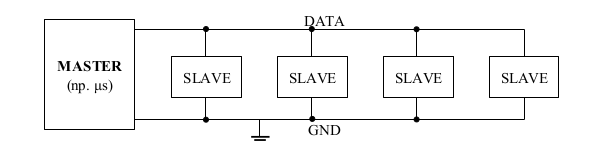
\includegraphics[scale=0.3]{graphics/idea.png}
\end{center}
\caption{Przykładowe połączenie urządzeń}
\label{schemonewire}
\end{figure}

Wyróżnia się urządzania typu Master (najczęsciej mikrokontroler) oraz Slave (peryferia).


\section{Podstawowe operacje}

\subsection{Inicjalizacja i reset}

Każda próba komunikacji urządzeń master i slave musi zacząć się od sekwencji składającej się z sygnału reset, wysyłanego przez master, po którym następuje sygnał obecności układu slave. Sygnał reset to wymuszony stan 0 trwający przynajmniej 480$\mu$s. Następnie master oczekuje na sygnał obecności innego urządzenia na linii. Następuje wówczas zwolnienie magistrali, co powoduje podciągnięcie jej do stanu wysokiego przez rezystor pull-up. Urządzenie slave wykrywa wówczas narastające zbocze lini i po upływie 15$\mu$s-60$\mu$s sygnalizuje swoją obecność poprzez wymuszenie stanu niskiego na okres 60$\mu$s-240$\mu$s.

\begin{figure}[!h]
\begin{center}
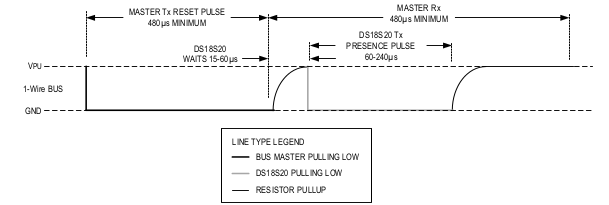
\includegraphics[scale=0.4]{graphics/init.png}
\end{center}
\caption{Diagram czasowy dla procedury inicjalizacji}
\label{inititming}
\end{figure}

\subsection{Zapis i odczyt}
\subsubsection{Zapis bitu}
Operacje zapisu bitu realizowane są w ściśle określonych slotach czasowych. Długość jednego slotu wynosić zwykle 60$\mu$s. Próbkowanie dokonywane jest mniej więcej w środku slotu celem uodpornienia na błędy. Pomiędzy kolejnymi operacjami wymagana jest przynajmniej 1$\mu$s odstępu.

Zapis rozpoczyna się wysterowaniem linii danych przez master na poziom niski. Zapis 0 wymaga utrzymania jej w tym stanie przez cały slot. Zapis 1 jest nieco bardziej skomplikowany. Master musi w czasie nie dłuższym niż 15$\mu$s, ale nie krótszym niż 1$\mu$s zwolnić magistralęm tak aby w momencie próbkowania (po 30$\mu$s od zbocza opadającego) była w stanie wysokim. 

\subsubsection{Odczyt bitu}
Odczyt bitu również wymaga 60$\mu$s slotu oraz 1$\mu$s przerwy. Odczyt rozpoczyna się wymuszeniem przez master stanu niskiego na linii danych na czas nie krótszy niż 1$\mu$s i zwolnienie jej (powrót do stanu wysokiego). Po tym sygnale sterowanie linią przejmuje urządzenie slave, wysyłające bit 0 lub 1. Slave po wykryciu zbocza opadającego wymusza stan niski (dla 0) lub utrzymuje  wysoki (dla 1) linii danych. Sygnał musi być wtedy spróbkowany przez master. Przed upłynięciem czasu końca slotu maigistrala zostaje zwolniona przez slave, co powoduje jej powrót do stanu wyokiego.

\begin{figure}[!h]
\begin{center}
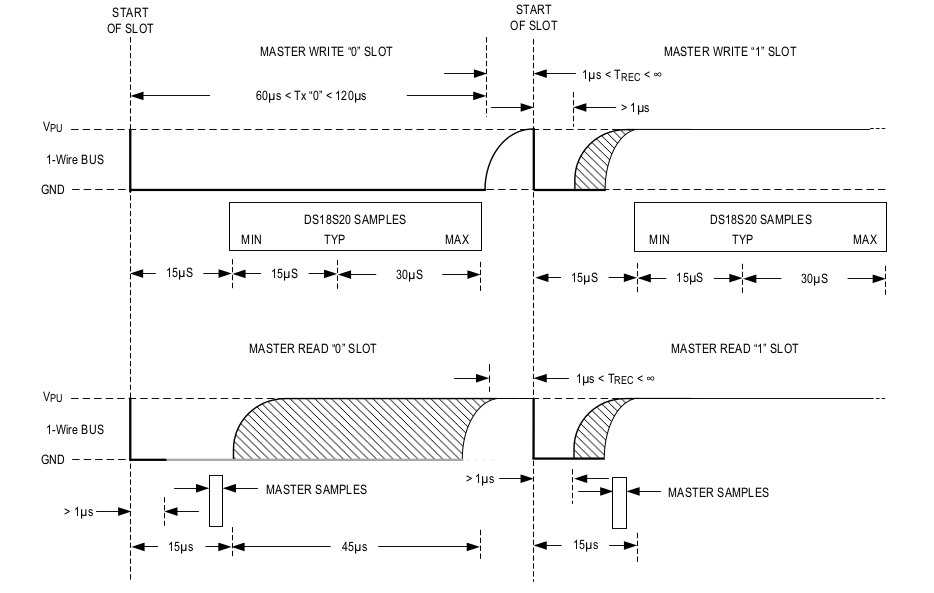
\includegraphics[width=14cm]{graphics/slots.png}
\end{center}
\caption{Diagramy czasowe dla procedury zapisu i odczytu}
\label{slotsitming}
\end{figure}

\section{Implementacja podstawowych operacji}

Za realizację podstawowych operacji odpowiada moduł BusController. 

\begin{figure}[!h]
\begin{center}
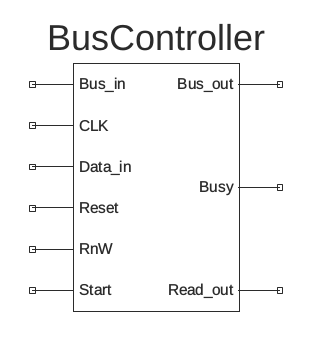
\includegraphics[height=5cm]{graphics/bus_controller_sym.png}
\end{center}
\caption{Moduł obsługi podstawowych operacji bitowych}
\label{bus_controller_sym}
\end{figure}

Poniżej przedstawiono schemat blokowy tego automatu.

\begin{figure}[!h]
\begin{center}
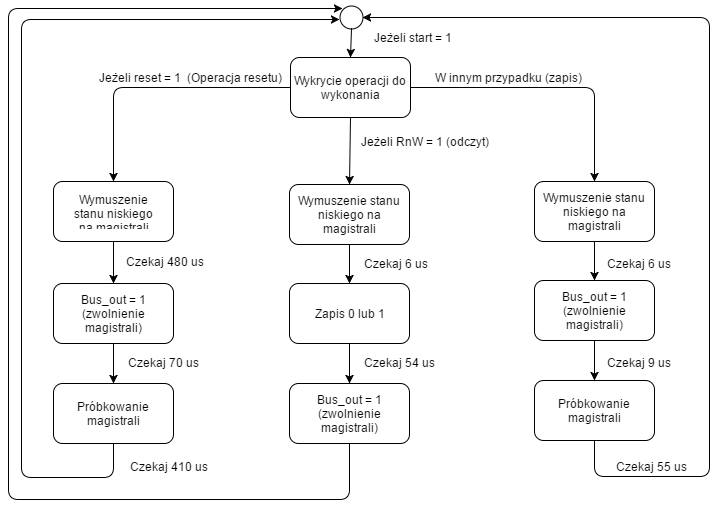
\includegraphics[width=15cm]{graphics/bus_controller_fsm.png}
\end{center}
\caption{Maszyna stanów BusController}
\label{bus_controller_fsm}
\end{figure}

Poprawna obsługa magistrali wymaga jej zwalniania poprzez ustawienie w stan wysokiej impedancji (podciągnięcie do Vcc przez rezystor pull-up). Służy do tego element IOBuf. Podanie logicznego zera na wejście T otwiera bufor wyjściowy i przekazuje sygnał podawany na pin I (GND - Logiczne 0). Logiczne 1 na wejściu T ustawia linie w stanie wysokiej impednacji (zwalnia magistralę). Pin O służy do odczytu stanu magistrali.

\begin{figure}[!h]
\begin{center}
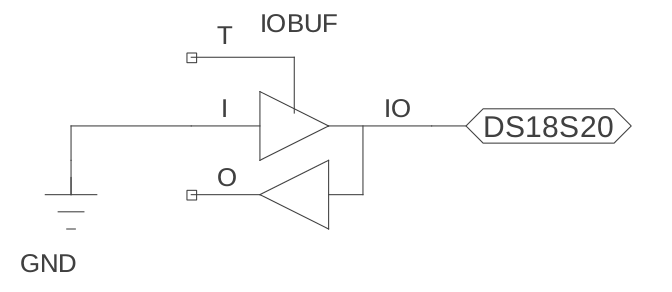
\includegraphics[scale=1.4]{graphics/io_buf_sym.png}
\end{center}
\caption{Symbol IOBuf}
\label{iobuf_controller_sym}
\end{figure}

\section{Transmisja bajtu}

Komunikacja master - slave jest dwukierunkowa. Dane przesyłane są w formie bajtów, kolejność bitów określa zasada najpierw najmłodszy. 

\section{Implementacja transmisji bajtu}

Transmisja bajtu realizowana jest poprzez następny moduł - ByteModule. 

\begin{figure}[h!]
\begin{center}
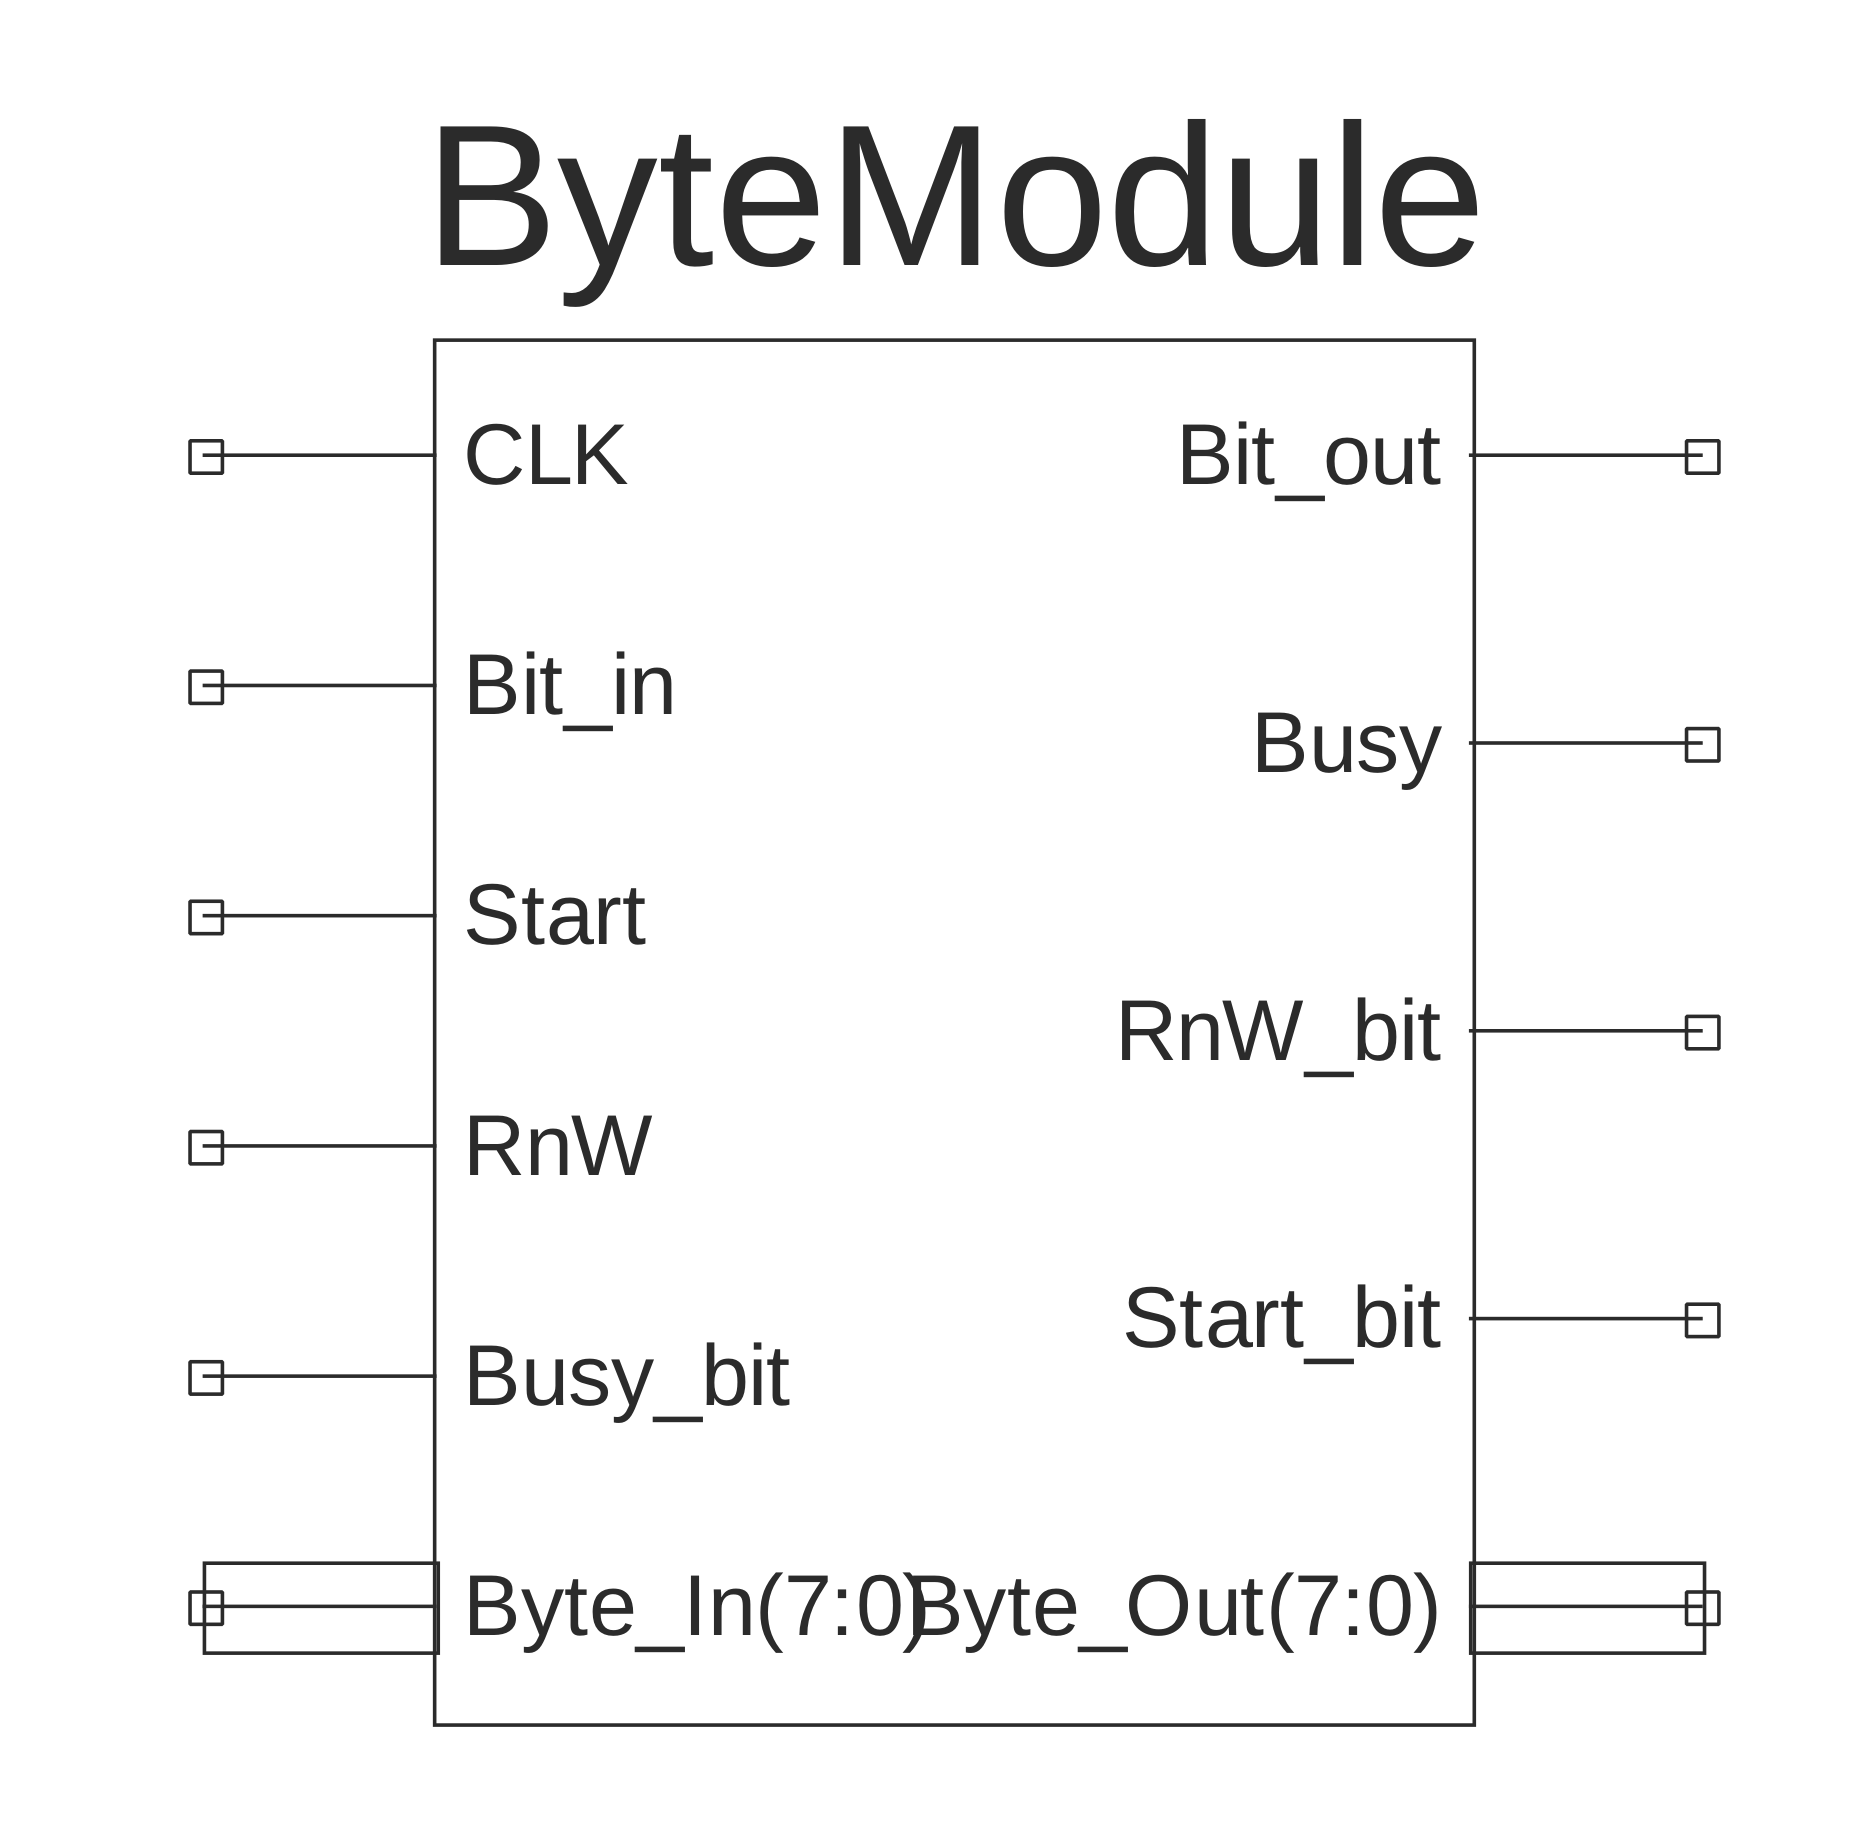
\includegraphics[height=5cm]{graphics/byte_module_sym.png}
\end{center}
\caption{Moduł transmisji bajtu}
\label{byte_module_sym}
\end{figure}

Automat zawiera po 4 stany na odczyt i zapis oraz jeden stan oczekiwania na sygnał startu.

\begin{figure}[!h]
\begin{center}
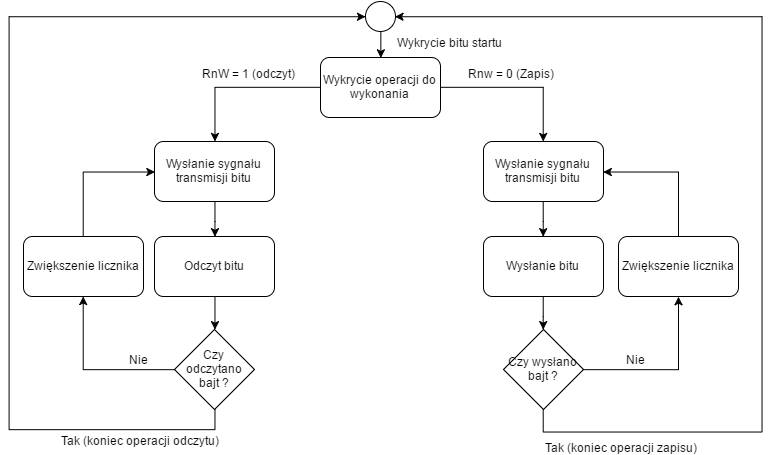
\includegraphics[width=15cm]{graphics/byte_module_fsm.png}
\end{center}
\caption{Maszyna stanów ByteModule}
\label{bte_module_fsm}
\end{figure}


\section{Sekwencja konwersji i odczytu temperatury}

Aktualna oczyt teperatury zapisany jest w dwóch pierwszych bajtach pamięci Scratchpad. Po poprawnej inicjalizacji czujnika DS18S20 ich zawartość odpowiada temperaturze +85$^\circ$C. Sekwencję polecń wymaganych do konwersji i odczytu 

\section{Implementacja konwersji i odczytu temperatury}
\section{Algorytm double dabble}
\section{Implementacja double dabble}
\end{document}